\documentclass[10pt]{article}
\usepackage{icmlko}

\icmlmeta{IP 파운데이션 월드모델}{319}{손잡이를 찾았는데 배분일 뿐이다}{도메인 무게를 같게 하니 아이돌이 0.24 오르고 도서가 0.17 내린다 --- 예측 그대로, 그리고 배포는 거절}

\begin{document}

\twocolumn[
\icmlheader

\begin{abstract}
노트 318이 ``몫이 풀링 효과의 크기를 정한다''를 $\rho_s{=}{-}0.943$ 으로
냈는데, 그 훑기는 \emph{도메인을 빼서} 몫을 올렸다 --- 자료를 버린다.
\textbf{자료를 다 쓰면서 몫만 올리는 손잡이}가 있다: \texttt{sample\_weight}
로 도메인마다 총 무게를 같게 준다(지금 0.15\%$\sim$25.5\% $\to$ 전부 9.09\%).
재기 전에 예측을 적었다. \textbf{맞았다} --- \textbf{아이돌 $+$0.2420}
($t{=}{+}3.11$, 예측 0.35$\sim$0.55 구간에 0.3432 로 착지) · \textbf{판
$-$0.0147}($t{=}{-}2.70$, 예측 $-$0.005$\sim$$-$0.02) · \textbf{도서
$-$0.1661}($t{=}{-}3.76$, 방향 예측대로). \textbf{판으로는 지고 아이돌로는
이긴다} --- 미리 적은 그대로이고, 노트 317의 ``판이 도메인 이득을 구조적으로
못 본다''의 재확인이다. 그리고 \textbf{가중이 풀링을 되돌린다} ---
풀링 이득과 가중 이득의 피어슨이 \textbf{$-$0.888} 이고, 효과 크기가
몫과 $\rho_s{=}{-}0.767$ 로 붙는다. \textbf{노트 318의 법칙이 다른 손잡이로
확인됐다.} 그런데 \textbf{배포는 거절이다} --- 판이 검출 문턱(0.011)을 넘게
내리고 도서($-$3.76)와 애니($-$2.84)가 도메인 문턱을 넘게 나빠진다.
\textbf{손잡이는 점수를 만들지 않고 옮긴다} --- 아이돌이 얻는 $+$0.24
$\times$ 25행보다 도서가 잃는 $-$0.17 $\times$ 163행이 크다.
\end{abstract}
]

\section{자료를 안 버리는 손잡이}

노트 318이 풀을 작은 도메인부터 키우며 아이돌을 훑어 $\rho_s{=}{-}0.943$ 을
냈다. 그 훑기에는 두 가지가 얽혀 있다 --- \emph{몫}과 \emph{누구를 넣었나}.
작은 것부터 넣었으므로 갈리지 않는다.

\paragraph{가중은 갈라 준다} \texttt{sample\_weight} 로 각 도메인의 학습 행
총 무게를 같게 준다($w_i = (N/K)/n_d$). \textbf{자료는 다 쓰고 몫만 바꾼다.}
모형 종류도 안 바꾼다(F18 의 \texttt{fit} 에서 가중만 넣는다).

\begin{center}\footnotesize
\begin{tabular}{lrr}
\hline
& 지금 몫 & 가중 뒤 \\
\hline
세계애니 & 25.5\% & 9.09\% \\
웹툰 & 20.3\% & 9.09\% \\
$\vdots$ & & \\
도서 & 0.77\% & \textbf{9.09\%} \\
아이돌 & 0.52\% & \textbf{9.09\%} \\
팝업 & 0.15\% & \textbf{9.09\%} \\
\hline
\end{tabular}
\end{center}

\section{예측한 대로다}

\begin{figure*}[t]
\centering
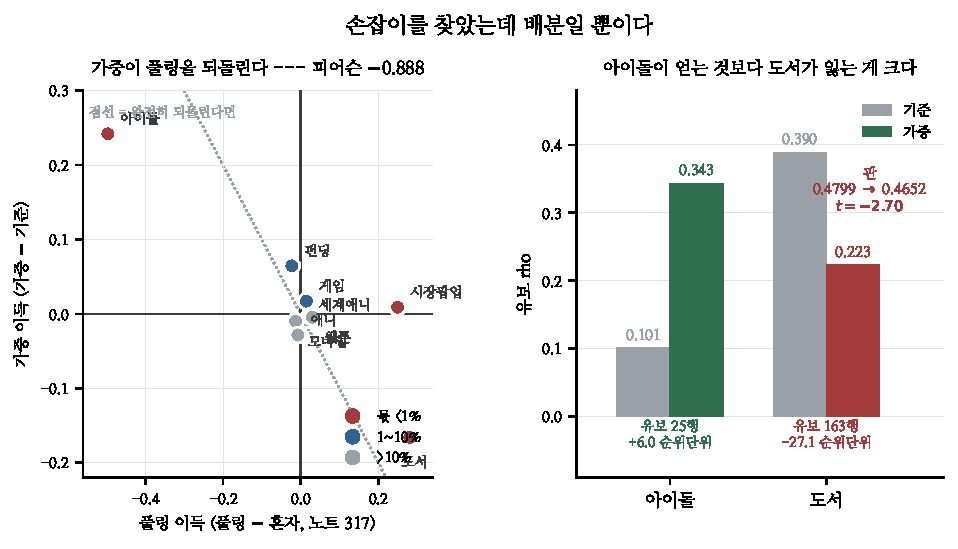
\includegraphics[width=\textwidth]{figs/realloc.pdf}
\caption{왼쪽 --- 풀링 이득(노트 317)과 가중 이득. 오른쪽 --- 아이돌과 도서.}
\end{figure*}

\begin{center}\footnotesize
\begin{tabular}{lrrrl}
\hline
도메인 & 기준 & 가중 & 차 & $t$ \\
\hline
게임 & 0.5893 & 0.6064 & $+$0.0171 & $+$1.18 \\
\textbf{도서} & 0.3895 & 0.2234 & \textbf{$-$0.1661} & \textbf{$-$3.76} \\
모바일 & 0.5464 & 0.5365 & $-$0.0099 & $-$1.23 \\
세계애니 & 0.5475 & 0.5394 & $-$0.0081 & $-$0.73 \\
시장팝업 & 0.4098 & 0.4186 & $+$0.0088 & $+$0.22 \\
\textbf{아이돌} & 0.1012 & 0.3432 & \textbf{$+$0.2420} & \textbf{$+$3.11} \\
\textbf{애니} & 0.4764 & 0.4479 & \textbf{$-$0.0284} & \textbf{$-$2.84} \\
웹툰 & 0.4614 & 0.4569 & $-$0.0045 & $-$0.48 \\
팝업 & 0.4062 & 0.4032 & $-$0.0030 & $-$0.05 \\
펀딩 & 0.2536 & 0.3181 & $+$0.0645 & $+$1.09 \\
\hline
\textbf{판} & 0.4799 & 0.4652 & \textbf{$-$0.0147} & \textbf{$-$2.70} \\
\hline
\end{tabular}
\end{center}

\begin{center}\footnotesize
\begin{tabular}{lll}
\hline
& 미리 적은 것 & 나온 것 \\
\hline
아이돌 & $+$0.35 $\sim$ $+$0.55 & \textbf{0.3432} (구간 하단) \\
도서 & $-$0.05 $\sim$ $-$0.15 & $-$0.1661 (조금 넘음) \\
큰 넷 & $\pm$0.02 & $-$0.028 $\sim$ $+$0.017 \\
판 & $-$0.005 $\sim$ $-$0.02 & \textbf{$-$0.0147} \\
\hline
\end{tabular}
\end{center}

\textbf{시장팝업만 예측을 벗어났다} --- ``내린다''고 적었는데 $+$0.0088
($t{=}0.22$)로 안 움직였다. 학습 101행이라 9\% 무게에서 오히려 잘 맞는
자리일 수 있다.

\section{가중이 풀링을 되돌린다}

\begin{center}\small
\begin{tabular}{lr}
\hline
풀링 이득 대 가중 이득 & 피어슨 \textbf{$-$0.888} \\
& 스피어만 $-$0.533 ($p{=}0.14$) \\
몫(log) 대 $|$가중 이득$|$ & 스피어만 \textbf{$-$0.767} \\
\hline
\end{tabular}
\end{center}

\begin{center}\footnotesize
\begin{tabular}{lrr}
\hline
& 풀링 이득 $|\cdot|$ & 가중 이득 $|\cdot|$ \\
\hline
몫 10\% 위 넷 & 0.0161 & 0.0127 \\
몫 1\% 아래 셋 & \textbf{0.3421} & \textbf{0.1390} \\
\hline
\end{tabular}
\end{center}

\textbf{같은 법칙이다.} 몫이 작은 도메인만 크게 움직이고, 움직이는 방향은
풀링이 준 것을 되돌리는 쪽이다. 아홉 중 여섯이 부호가 반대이고 둘은 잡음
안이며 하나(애니)만 같은 부호다. \textbf{노트 318 을 다른 손잡이로 확인했다}
--- 도메인을 버리지 않고서도 같은 곡선을 탄다.

\section{그런데 배포는 거절이다}

\begin{center}\footnotesize
\begin{tabular}{ll}
\hline
배포 규칙(노트 275 · 282) & \\
\hline
① 판이 미결정 띠 안 & \textbf{탈락} ($-$0.0147 · 문턱 0.011) \\
② 나빠진 도메인 $|t|{>}2.81$ & \textbf{탈락} (도서 $-$3.76 · 애니 $-$2.84) \\
\hline
\end{tabular}
\end{center}

\textbf{둘 다 탈락이다.} 손잡이는 찾았고 법칙도 확인했지만 \textbf{이대로는
안 쓴다.}

\paragraph{왜 판이 지나} \textbf{점수를 만드는 게 아니라 옮기기} 때문이다.

\begin{center}\footnotesize
\begin{tabular}{lrrr}
\hline
& 차 & 유보 & 차$\times$유보 \\
\hline
아이돌 & $+$0.2420 & 25 & $+$6.1 \\
도서 & $-$0.1661 & 163 & \textbf{$-$27.1} \\
애니 & $-$0.0284 & 606 & \textbf{$-$17.2} \\
펀딩 & $+$0.0645 & 80 & $+$5.2 \\
\hline
\end{tabular}
\end{center}

\textbf{아이돌이 얻는 것보다 도서와 애니가 잃는 것이 여섯 배다.} 유보 25행
짜리를 살리려고 163행과 606행을 내주는 셈이다.

\section{그러면 이 손잡이는 무엇에 쓰나}

\begin{center}\footnotesize
\begin{tabular}{ll}
\hline
쓸 데 & \\
\hline
\textbf{절충을 눈에 보이게} & 아이돌 $+$0.24 의 값이 도서 $-$0.17 \\
\textbf{목표가 바뀌면} & 얇은 도메인이 목적이면 이 쪽이 옳다 \\
\textbf{부분 가중} & 전부 같게가 아니라 $n^{\alpha}$, $\alpha{<}1$ \\
\hline
안 되는 것 & \\
\hline
지금 판을 이걸로 & 규칙 둘 다 탈락 \\
\hline
\end{tabular}
\end{center}

\textbf{판 $\rho$ 는 유보 행으로 가중하므로 이미 하나의 선택이다} --- ``큰
도메인이 중요하다''는 선택. 가중은 그 선택을 뒤집는 손잡이이고, 지금 목표
아래에서는 지는 쪽이다. \textbf{목표가 ``얇은 도메인에서도 쓸 만한 모형''이면
같은 실험이 이기는 쪽으로 읽힌다.}

\paragraph{남은 것}
\begin{center}\small
\begin{tabular}{ll}
\hline
갈래 & 왜 \\
\hline
$n^{\alpha}$ 부분 가중 & 절충 곡선을 그린다 \\
얇은 것끼리 따로 풀 & 큰 쪽을 안 건드린다 \\
도서는 왜 그렇게 잃나 & 풀에 제일 많이 기댔다 \\
선형에서도 같은가 & F6 은 탐욕 분할이 없다 \\
\hline
\end{tabular}
\end{center}

\paragraph{규약} \textbf{손잡이를 찾았으면 그것이 만드는지 옮기는지 물어라.}
아이돌 $+$0.24 는 이 판에서 오늘 잰 것 중 제일 큰 도메인 이득인데
\textbf{판은 내려간다.} 차$\times$유보로 세면 왜인지 즉시 보인다.
그리고 \textbf{예측을 적어 두면 맞은 것과 벗어난 것이 같이 보인다} ---
넷 중 셋이 구간 안이고 시장팝업 하나가 벗어났다. \textbf{벗어난 하나가
다음 물음이다.}

\end{document}
